\section{Introduction}

Software packages are widely used in software development to improve productivity. However, usage of software packages can be difficult, which is widely known as the \emph{dependency hell}.

This section briefly explains why usage of software packages is difficult and the motivation for experimenting a new algorithm.

\subsection{Why usage of packages is difficult}
Usage of software packages is complicated by \emph{package versioning}, \emph{transitive dependency} and \emph{complex dependency constraints}.

Software packages evolve over time, some supported features might no longer be supported afterwards, some interface might be changed or deprecated later. Software packages are usually versioned by some \emph{versionning scheme} to clearly mark the changes in each version. Users of a package should know the exact version that's been used to make sure it supports all the required features and the documentation conforms to the specific version.

Software package dependency is transitive. If a package $x$ depends on a package $y$, and $y$ depends on a package $z$, then $x$ depends on $z$. Though developers specify the dependencies as a flat list, it usually expands to a complex directed graph.

Dependency specification requires the support of complex constraints, like \emph{fuzzy version constraints}, \emph{excludes in transitive dependency}, \emph{intransitive dependency}, etc. For example, a project may need to specify fuzzy version constraints, such as $(, 1.0.0]$, $[1.5.2, 1.6.0)$, etc. Sometimes there's the need to exclude a specific package from all later transitive dependencies or to mark a dependency as intransitive.

The complexity in software packages may lead to two problems -- one is \emph{conflict}, the other is \emph{missing dependency}. Usually, only one version of a package can be used in the same project. If a project transitively depends on two different versions of the same package, then there's a \emph{conflict}. On the other hand, if a project depends on a package that can't be found, then there's a \emph{missing dependency}.

The complexity with the usage of packages necessitates tools to automatically check whether a dependency specification can be satisfied or not. More concretely, a dependency manager has to check that for a given dependency specification (1) whether there exists conflicts or missing dependencies; (2) if there's no error, generate an optimal set of packages so that the dependency constraints of the specification and of each package in the solution set are satisfied.


\subsection{Motivation of the project}

In the Java world, Maven\footnote{\url{https://maven.apache.org}} and Ivy\footnote{\url{http://ant.apache.org/ivy/}} are the two most widely used dependency management tools.

The common problem with Ivy and Maven is that they resort to conflict resolution unnecessarily even when the specification is satisfiable with no conflicts. This is better illustrated with Figure \ref{fig:introuction:underconstraint}, where the rectangles represent versioned packages, and the rounded rectangles represent dependency constraints.  As we can see in the graph, the project depends on the package A and B directly, and they in turn depend on the package C.

\begin{figure}[ht]
  \center
  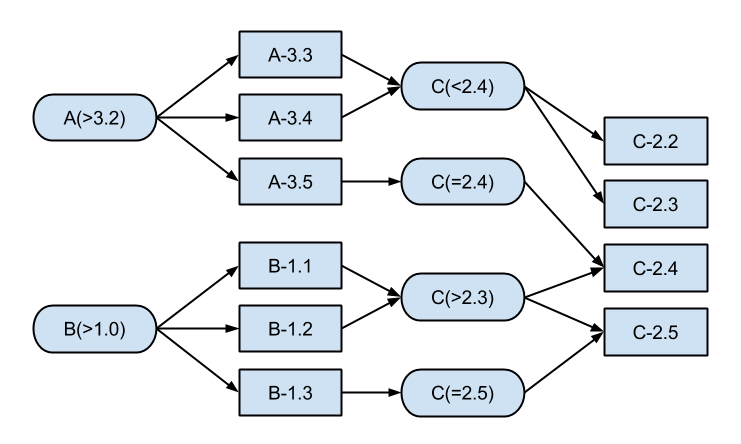
\includegraphics[width=14cm]{img/introduction/underconstraint.png}
  \caption[An example dependency graph]{An example dependency graph \label{fig:introuction:underconstraint}}
\end{figure}

It's obvious that the dependency graph in Figure \ref{fig:introuction:underconstraint} has a solution set $\{(A, 3.5), (B, 1.2), (C, 2.4)\}$. However, both Maven and Ivy would think there's a conflict on the package $C$, and the conflict manager would be called to resolve the conflict. Depending on the setting of the conflict manager, usually $(C, 2.5)$ will be chosen, which is incorrect! This behavior is documented on Ivy official web site\footnote{\url{http://ant.apache.org/ivy/history/latest-milestone/principle.html}}:

\begin{quote}
  When the dependency module has been found, its ivy file is downloaded to the ivy cache. Then ivy checks if the dependency module has dependencies, in which case it recursively traverses the graph of dependencies.

  All over this traversal, conflict management is done to prevent access to a module as soon as possible.
\end{quote}

The popular build tool Gradle\footnote{\url{https://gradle.org}} has the similar problem, as documented in section \emph{50.7. How dependency resolution works} on their official site\footnote{\url{https://docs.gradle.org/current/userguide/dependency_management.html}}.

In Scala, Sbt\footnote{\url{http://www.scala-sbt.org}} depends on Ivy to resolve dependencies, so it inherits the problem. It produces confusing resolution results to users sometimes. The motivation for this project is to experiment with a new algorithm based on SAT solvers to avoid this problem. If proved feasible, sbt can drop the dependency on Ivy and use the new algorithm in the future to avoid the problem.

\subsection{Contributions of the project}

This project has two major contributions. First, the successful application of SAT solvers to dependency resolution both for the Maven and the Ivy ecosystem. There has already been many applications of SAT solvers in dependency management\cite{mancinelli2006managing, berre2009dependency, vouillon2013software}, but implementation of the method for the Maven and Ivy ecosystem in the context of software development is a new attempt. This project demonstrates that this approach is feasible.

Second, based on argumentative reasoning, this report proposes the separation of project specification and artifact specification, and a restriction on the features of artifact specification. These reflections might be helpful for future ecosystem designers.
